% -*- fill-column: 85; -*-
%!TEX root = ../dissertation.tex

\section{Implementation}
\label{s:impl}

We prototyped \AvA on Linux kernel~4.14.0 with QEMU~3.1.0 and LLVM~7.0.
Our resource management modifications to the KVM hypervisor took 1,500~LoC.
We modified the QEMU \emph{virtio-vsock} device and the corresponding \emph{vhost-vsock} host driver to enable interposition (\S\ref{s:impl_mediation}).
The para-\vdev, which is used for both interposition and transport, was built as a QEMU display adapter (500~LoC). The guest driver is 500~LoC long, each transport channel is about 400~LoC on average, the \CAvA was implemented in 3,200~LoC of Python code. Other libraries accounted for 2,000~LoC.

\subsection{Transport}

\begin{comment}
\begin{figure}[!t]
	\centering
	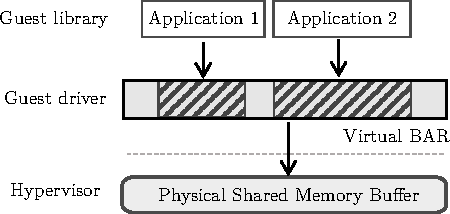
\includegraphics[width=.75\linewidth]{ava/images/memory_hierarchy.pdf}
	\caption{Three-level virtual memory structure. The \vdev BAR is managed by guest driver.
    \cjr{not sure this is helping, but needs to shrink if we keep it.}
    }
	\label{fig:memory_hierarchy}
\end{figure}
\end{comment}

\AvA supports several interchangeable transports, allowing it to support disaggregated hardware via \emph{sockets}, as well as local execution via guest-\worker \emph{shared memory}.
% The transport handles two types of payloads: commands which contain opaque arguments and metadata for calls (e.g., thread ID and function ID) and data which contains buffers referenced from the arguments (e.g., bulk data).
% The \AvA prototype implements two types of transports.
The \emph{socket} transport uses either a TCP/IP network socket or an inter-VM socket (VSOCK) to transport commands and data.
The socket layer copies data multiple times, and incurs queuing delays.
%This transport is currently only used to connect different computers.
% We are currently investigating supporting RDMA.
% , but this is future work.
\emph{Shared memory} provides efficient data transfer when the guest and the \worker are on the same physical machine.
% It uses three-level shared virtual memory management, shown in
%Figure~\ref{fig:memory_hierarchy} shows how this transport is built.
The hypervisor exposes a contiguous virtual buffer to the VM through the \vdev PCIe BAR (base address register).
The guest para-virtual driver manages the virtual BAR and assigns a partition to each guest application.
% AMP: speculation
% More advanced memory management could be used in the future.
% for example, the parameter blocks may be relocated in the BAR to reduce the external fragmentation.
\AvA uses the shared buffer to transport buffers to the \worker,
but still uses a socket (currently VSOCK) to transport commands to retain hypervisor interposition.
% Because the buffers are virtual memory they do not consume physical memory until they are used and thus can be over allocated without significant waste.

\begin{comment}
Comparing two transport channels,
the hypervisor-mediated shared memory is able to achieve peak memory copy performance (about 3.8~GB/s on the test machine) and requires at most one copy for data transfer (guest application to shared buffer).
However, Spinning on a memory location to implement a doorbell costs more CPU resources and requires complex synchronization algorithms.
VSOCK performance can be improved to nearly match memory performance~\cite{vsock-mergeable-rx},
but it would still increase the number of data copies and increasing performance would require modifications to the hypervisor and the guest and host kernels.
In this trade-off space,
the shared memory channel in \AvA combines socket channel for doorbell notifications and uses shared memory for bulk data transport.
\end{comment}

% AMP: This really isn't important. It's just a variant of the socket transport.
% \paragraphbe{Netlink} socket channel~\cite{netlink} is established for communications between hypervisor and services (manager and \workers).
% The hypervisor offers interfaces to receive invocations' execution statistics from \workers and provide scheduling information,
% enforcing resource policies (\S\ref{s:policy}).
% The commands sent from either manager or \workers are usually forged automatically by \CAvA (\S\ref{s:compiler}),
% and flagged as \AvA internal commands.

% AMP: This may be worth using in the record-and-replay implementation section.
% \paragraphbe{Recording} channel is used for log-and-replay migration support (\S\ref{s:migration}).
% To support object-level migration, the original \worker in \AvA must be able to record a selected set of invocations and capture the states of API objects.
% The destination \worker must be able to read the recorded invocation logs and object states to restore the context.
% \AvA eases the difficulty in writing such a log-and-replay channel,
% where the source worker writes the record to a disk file or socket channel, and the destination reads the file or socket to retrieve the log.

\subsection{Hypervisor Interposition and Mediation}
\label{s:impl_mediation}

\AvA enables hypervisor mediation by interposing the transport channel.
 % to be mediated by the (local) hypervisor.
% We achieve this mediation with a para-\vdev exposed to the VM.
We extended QEMU \emph{virtio-vsock}~\cite{virtio,virtio_vsock} (a
%zero-configuration
host/guest communication device) to build the virtual device.
% with the interface shown in Figure~\ref{fig:memory_hierarchy},
% the prototype builds the \vdev on top of virtio-vsock device,
The corresponding \emph{vhost-vsock} host driver was extended to perform interposition during packet delivery.
% \aak{hyu, please check my changes}
% However, the hypervisor could use this interposition point, for example, to validate commands and buffers before forwarding the command.

When forwarding an API call, the command is always sent on the modified VSOCK channel, while the argument buffer can be transferred via either VSOCK or guest---\worker shared memory.
Transferring the command via VSOCK provides a doorbell to the router---%
the router then schedules the invocation based on resource limits.
% reported by the \worker.
The \worker and guest application have unfettered access to the shared memory, but the \worker does not know what the requested operation is or where the buffers are until the hypervisor forwards the command.

\subsubsection{Policies in eBPF}
\label{s:bpf}

\AvA supports policies written as eBPF (Extended Berkeley Packet Filter~\cite{bpf}) programs.
We defined a new eBPF program type
% \lstinline|BPF_PROG_TYPE_AVX_POLICY|
that can be loaded into KVM via \lstinline|ioctl|.
% In the prototype, the command doorbells are sent via VSOCK and resource reports are sent via Netlink, and in the disaggregated scenario, both are sent via TCP or RDMA,
\AvA reuses the same eBPF instruction set as socket filtering,
and leverages the unmodified LLVM compiler to compile the eBPF program.
The eBPF verifier had to be modified to verify the memory accesses of the new type of program.
We provide helper functions for \AvA eBPF programs.
% As running in the BPF VM,
Leveraging eBPF allows \AvA to take advantage of eBPF program verification at a very low cost (4.3\% of \AvA's internal overhead).
% benefit from the  for the security purpose.
% \hyu{The overhead of BPF program execution is negligible compared with the whole API execution time. It does take long time compared with the native code: The schedule program takes 2~us on average, consume program takes 300~ns (for every 20 invocations in a batch). For comparison, the overhead of forwarding an invocation without arguments is about 47~us (marshal 5us, unmarshal 9us, scheduling <1us, memcpy 200 bytes * 4 => 6us, vsock 8us, others 12us). So it increases the total overhead by (2+0.3/20)/47=4.3\%.}

The current implementation computes resource utilization in the \worker and then reports this utilization to the hypervisor.
This simplifies the implementation somewhat, but will be changed in the future so that resources tracking can be performed fully in the hypervisor.


% Each forwarded invocation is separated into a doorbell message and argument buffers.
% The doorbell message is always sent via vsock channel, which is intercepted and interposed by hypervisor before it is placed into the \worker's RX virt-queue.
% The argument buffers are transferred via different channels, e.g., vsock, shm, TCP, etc.
% }

\begin{comment}

% The design can be ported to other OS and platforms easily with the flexible disaggregated components.
\aak{does this belong in a section on hypervisor mediation?}\cjr{I think it goes here, but I think maybe it also gets deleted.}
The \AvA developer can develop new mediated channels into the \AvA transport,
and the design generalizes well to other hypervisors.
For example, our first prototype of \AvA was built on Xen hypervisor where virtio-vsock was introduced in version 4.9.
On VMware ESXi, the mediated VSOCK channel can be replaced with VMCI Sockets (vmw-sock).
\end{comment}

\subsubsection{Scheduling}
\label{sub:scheduling}
\AvA provides a weighted fair queuing (WFQ) scheduler, with two rate control algorithms.
%, as an individual Linux kernel module.
% and instructs the router to trigger the defined functions at the scheduling points.
% \AvA implements .
Each VM $v$ sharing the device is configured with one share $s_v$.
$v$'s average device time usage is $L_v=s_v/\sum_{v\in V} s_v$, where $V$ is the set of running VMs.
VM~$v$'s device utilization time is accumulated into $T_v(t)$ in the time window $[t, t+1)$.
If a VM's device usage time exceeds its share $s_v$,
% namely, $$T_v(t)/\sum_{v\in V} {T_v(t)} > L_v,$$
API calls from $v$ will be postponed until its utilization proportion becomes lower than the threshold.
The scheduling window is 500~ms (or the interval between two adjacent calls),
and device utilization is updated upon every API completion.
\AvA supports the following algorithms:

\paragraphbe{Fixed-rate polling} where the delay is a fixed interval $d$ (usually longer than the time window).

\paragraphbe{Feedback control} where the adaptive delay, $d_v(t)$, is computed by the additive-increase multiplicative-decrease (AIMD) algorithm~\cite{aimd} below ($a=1$~ms and $b=1/2$; see \S\ref{s:eval_rate_limit}).

\[
d_v\left(t+1\right)=\begin{cases}
d_v\left(t\right)\times b, &\textrm{if VM $v$ exhausted its share}\\
d_v\left(t\right)+a, &\textrm{otherwise}
\end{cases}
\]

\begin{comment}
\paragraphbe{Feedback control v2}
The $k$-th call is delayed by an adaptive amount of time $d_v(k)$.
The delay is computed by the moving average of the lengths of previous $n$ executed kernels from VM $v$,
i.e., $$d_v(k) = b\sum_{t=1}^nl_v(k-t).$$ $b$ is a coherence for which $0<b\le 1$.
\end{comment}

\subsection{Shadow Resources}
\label{s:multi_thread}
\label{s:shadow_buffer}

\AvA supports threading and long-lived buffers by shadowing them in the \worker.
The \worker spawns a shadow thread when a new guest thread makes its first API call, and reuses it for all future calls from that thread.
%All commands sent to the worker are tagged with their thread ID and dispatched to the appropriate shadow thread in the \worker.
For synchronous calls, the guest thread will be blocked while the shadow thread executes the call.
Shadow threads are destroyed when the original thread is destroyed or when the guest application exits.
%For buffers,
Similarly, the worker allocates a new shadow buffer when it is first notified of a buffer annotated with a long lifetime and
% The annotations cause \AvA to use shadow buffers in the \worker which correspond to guest application buffers.
deallocates it when the application calls a function annotated with \lstinline@deallocates@.
Reverse shadows, guest library buffers, and threads which shadow an \worker resource, are supported in the same way.
% \cjr{I want to delete this paragraph, but I can't even convince myself I understand the first sentence. Let's discuss.}

\subsection{Callbacks}
\label{s:callback}

When an API registers a callback, the guest library stores both the original application \texttt{userdata/tag} value and the function pointer in a buffer.
This buffer is then supplied as the \texttt{userdata} argument to the \worker.
The \worker registers a generated stub function with the accelerator API.
When the API framework calls the stub in the \worker, a callback is made to the guest library with the guest library buffer as the \texttt{userdata} argument.
The guest library finally extracts the original application \texttt{userdata} value and function pointer and performs the call back into application code.
The call to the guest library uses the same protocol as calls to the \worker, so all features of \AvA apply to callbacks.
For example, callbacks block the \worker thread that called them if the callback is synchronous.


% AMP: We never did this, and it's pretty well known coherence tricks.
% \subsection{Memory mapping}
% \AvA supports mapped memory by maintaining a shadow memory copy in the \worker.
% Both original and shadow memory are write-protected and associated with a dirty bit when allocated.
% The dirty bit is set when any change is made to the memory region;
% the dirty memory is transferred back to the guest application when the invocation is completed,
% or transferred to the \worker when any invocation references that memory region.
% This enables a memory to be mapped across physical servers,
% while the more perfect way is to establish shared memory with Intel Extended Page Table (or AMD Second Level Address Translation) on local executions.